\documentclass[12pt]{article}
\usepackage{graphicx}
\usepackage{epstopdf}
\usepackage[spanish]{babel}
\selectlanguage{spanish}
%\usepackage[english]{babel}
\usepackage[utf8]{inputenc}
\usepackage{hyperref}
\usepackage[left=3cm,top=3cm,right=3cm,bottom= 2.5cm,nohead,nofoot]{geometry}
\usepackage{braket}
\usepackage{datenumber}
\usepackage{textcomp}
\usepackage{chemfig}%figuras Quimica
\usepackage[version=4]{mhchem}%nombres compuestos quimicos
\title{Procedimiento para el Cálculo de los Perfiles de Estrés}
\begin{document}
\maketitle
\section{Procedimiento}
El siguiente procedimiento ha sido realizado para 5 réplicas de 400ns hechas sobre cada una de los siguientes sistemas: DMPG, DPPG, 1STX:128DMPG, 1STX:128DPPG, 15\%STX en DMPG, 15\%STX en DPPG, 15\%STXrígida en DMPG, 15\%STXrígida en DPPG.\\
\begin{itemize}

\item Se modificó el archivo .mdp fijando las opciones de número de pasos, \texttt{nst}, a 0. La opción de \texttt{coulombtype} se colocó como \texttt{Cut-off} y la distancia de cuttoff, \texttt{rcoulomb} se fijó a 2.0nm.\\

Luego se creó el archivo .tpr, mediante las herramientas de gromacs de la siguiente manera:

\item Se creó un archivo .ndx que contiene los grupos de la membrana y del solvente unido con los iones.
\item Los sistemas de membrana fueron trasladados 3.7 nm para los sistemas con STX. Para trasladarlos se utilizó el comando gmx edticonf de gromacs 2016.3 y posteriormente se convirtió a formato tpr. %, mientras que los sistemas de membrana pura han sido centrados en el centro de la membrana, valor encontrado alrededor de 4nm.
\item Con \texttt{trjconv -fit traslation...} se ajusta la membrana.


\item A partir del archivo trr se calculó el tensor de estrés a lo largo de la coordenada z. Sé usó el siguiente comando:\\
\texttt{gmx\_LS mdrun -s step7\_LS.tpr -rerun traj\_centered.trr -localsgrid 0.05}\\
\texttt{ -lsgridx 1 -lsgridy 1 -ols localstress.dat0}\\

La salida del comando es un archivo binario .dat0.\\

\item Tomando el archivo .dat0, se generó un archivo .txt qué contiene el tensor de estrés por cada coordenada z. Mediante la herramienta \texttt{tensortools} a estos valores se les aplica un filtro gaussiano de 2,3 y 4 desviaciones estándar. Sin embargo, fueron escogidos los valores con el filtro gaussiano de 2 desviaciones al considerando el hecho de que se descartaban los valores más atípicos del perfil de estrés, pero se conservaban las fluctuaciones propias del sistema.\\

\item Con el tensor de estrés filtrado, se calcula el perfil de estrés mediante la fórmula:
\begin{equation}
\Pi (z)=-(\sigma_{xx}+\sigma_{yy})/2+\sigma_{zz}
\end{equation}
\item El perfil de estrés es calculado para cada una de las réplicas. Con estos valores de perfil de estrés se realiza un promedio sobre todas las réplicas y se realiza una simetrización del perfil de estrés obtenido, es decir, se promedian las coordenadas que están a la derecha y a la izquierda del centro de la membrana.\\
\end{itemize}
\section{Resultado}

En la figura \ref{fig:stress2} aparecen los perfiles de estrés obtenidos para cada uno de los sistemas siguiendo los pasos anteriores:\\
\begin{figure}
\begin{center}
    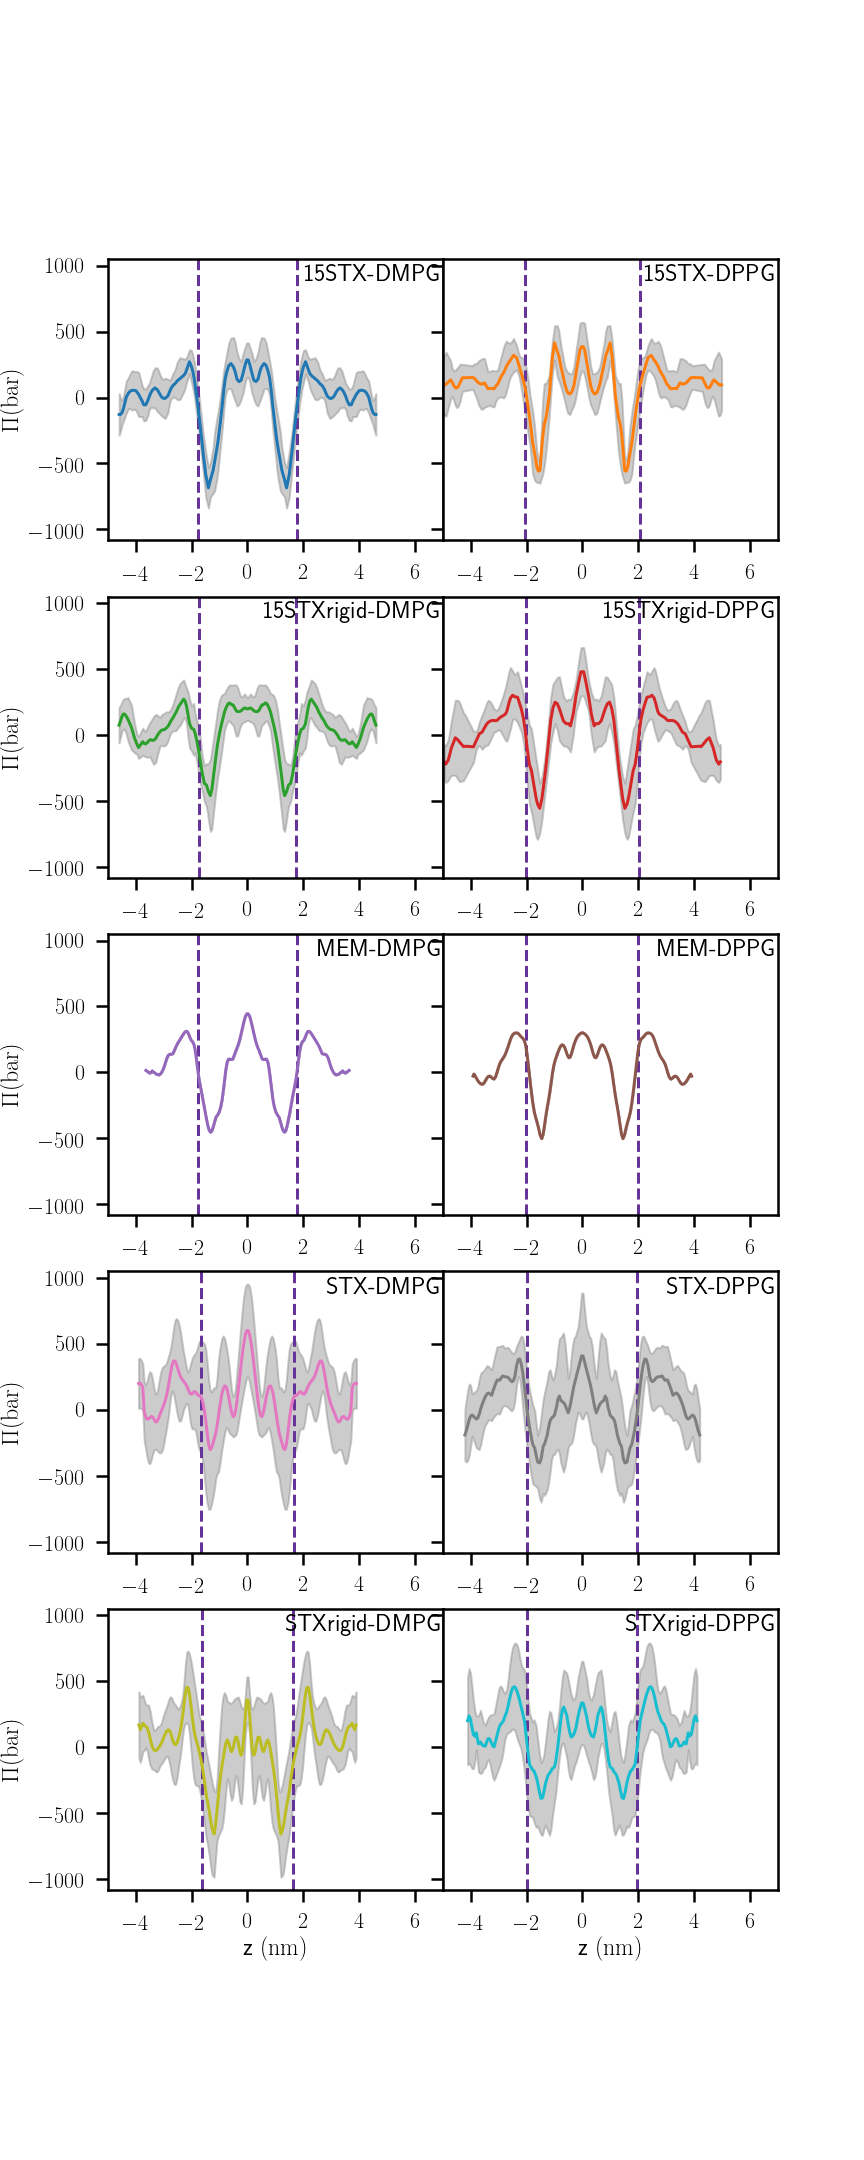
\includegraphics[scale=0.25,trim={0 6cm 0 9cm},clip]{../Plots/stress_profile_2_sym.png}
  \caption{Perfil de estr\'{e}s promediado para todas las r\'{e}plicas con un filtro gaussiano de 2. Las l\'{i}neas punteadas representan la posici\'{o}n de los grupos fosfato. }
  \label{fig:stress2}
\end{center}
\end{figure}
En la figura \ref{fig:stress2}, la l\'{i}nea punteada representa la posici\'{o}n de los grupos fosfato hallada mediante la herramienta de gromacs. Los dos m\'{a}ximos positivos del perfil de presi\'{o}n (picos positivos) corresponden a la posici\'{o}n de los grupos fosfato, esto es debido a la repulsi\'{o}n electrost\'{a}tica entre los f\'{o}sforos, los cuales poseen cargas ani\'{o}nicas, lo cual induce un trabajo positivo sobre el sistema, sin embargo, en la figura \ref{fig:stress2} la posici\'{o}n de los grupos fosfato de gromacs aparece desplazada hacia el centro respecto a los picos correspondientes.\\

Los dos m\'{i}nimos globales del perfil de presi\'{o}n (valles negativos) son valores negativos puesto que se deben a interacciones favorables entre los grupos apolares de la membrana debido a interacciones hidrof\'{o}bicas y que usualmente corresponden a interacciones en la interfaz hidrof\'{i}lica/hidrof\'{o}bica de la membrana. Los dos valles encontrados son acordes a los resultados de Vanegas et. al., ya que estos dos valles son m\'{a}s notorios cuando la membrana est\'{a} en la fase l\'{i}quida desordenada $L_{\alpha}$.\\

\end{document}
